% !TeX spellcheck = en_US
\documentclass[11pt, fleqn]{article}
%\usepackage{siunitx}
\usepackage{texfiles/SpeedyGonzales}
\usepackage{texfiles/MediocreMike}
\title{Changes to the Project Plan}
\date{}
\begin{document}
	\maketitle
	\noindent
	\vspace*{-1.4cm}
	\noindent
	\textbf{Project Title:} Fairness In Classification \newline \noindent
	\textbf{Group Members:} Oskar og Anders \newline  \noindent
	\textbf{Vejleder på engelsk:} Aase Feragen \noindent
	\\\\
	
		The project description overall has not changed much. The safety of AI has become ever more important throughout the thirteen weeks of work. This has been seen in countries such as China where cellphone data has been used to track and stop the spread of the Covid-19. 
		
	\section*{Gantt Chart}
	\noindent The original development of certain milestones and key achievements during the project writing process is visualized in the Gantt chart shown below. 
	\begin{figure}[H]
		\centering
		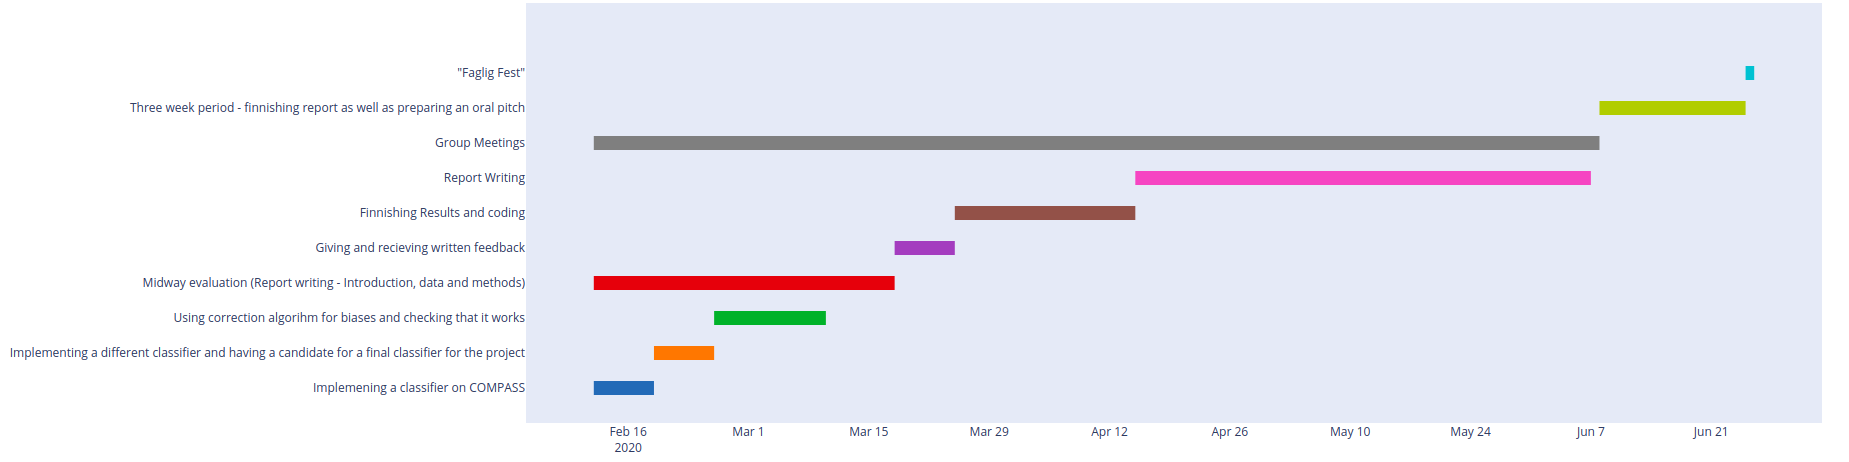
\includegraphics[width=\linewidth]{Gantt}
	\end{figure}

	Comparing this chart to the actual progress of the report writing, it is evident that it has been followed surprisingly well. As it seem wasteful to make strikingly similar classifers for the same task, the milestones of implementing the first classifier and creating the final classifer was merged into one. It also took longer, as some minor mistakes were made during the implementation. The bias correction algorithm took much longer to implement, as this turned out to be the same stage of the project as finishing results and coding. As such, this milestone was reached closer to the end of April than the middle of March. As we are in line with the further progression of the Gantt chart (and since one of the last major milestones is writing the rest of the report), this will continue to be a guide moving forward.
	
	\section*{Research Questions}
	The original research questions, in broad strokes, were to:
	\begin{itemize}
		\itemsep-0.1cm
		\item Figure out if the data from COMPAS is biased and which bias is prevalent
		
		\item Understand the effect of bias on a classification algorithm
		
		\item Implement equalized odds and equal opportunity from "Equality of Opportunity in Supervised Learning"
		
		\item Discuss, with focus on ethics, how the bias-corrected algorithm can be used fairly
	\end{itemize}
	
	Having gotten a more clear view of the project scope, it is clear that most aspects of the research questions are still relevant in the writing process moving forward. A minor change is that the first point will not take up much space in the final product, since this question can be answered using a few plots of the data.
	
	\section*{Learning Objectives}
	The original learning objectives were to:
	\begin{itemize}
		\itemsep-0.1cm
		\item Examine and understand bias in the COMPAS dataset
		\item Get an understanding of the process of writing and creating bigger group projects
		\item Limit the project in such a way as to only convey the necessary information
		\item Understand the ethics behind AI and ML models
	\end{itemize}
	
	After almost 13 weeks of writing the project, some of the learning objectives have taken a different direction. Bias understand has generally taken a backseat in order to instead put more focus on the important aspects – defining the used definitions of bias and using them practically to remove bias. Limiting the scope of the project will be important near the end of the writing process, but has not yet been given thought, since the general structure of the report, at this point in time, is still very open. The rest of the learning objectives still complement future work on the project.
	
	\section*{Cooperation Contract}
	Parts of the original plan outlined in the cooperation contract, which have later changed was to
	
	
\end{document}
